\documentclass{report}
\usepackage{amsmath}
\usepackage{fixltx2e}
\usepackage{fullpage}
\usepackage[super]{natbib}
\usepackage{graphicx}

\title{Linear Models Using Dysphonia to Predict Parkinson's Disease}
\author{Kevin Song, Matthew Bucci, Robert Puccinelli}
\date{\today}
\linespread{1.3}

\begin{document}
\maketitle

\section*{Introduction}

Motion, speech, and thought are so intrinsic to our being that it seems impossible to imagine living without them. The world, however, is indifferent to our beliefs.
In North America alone, over one million people are affected with Parkinson's Disease (PD), a neurodegenerative disorder which profoundly affects the central nervous system.
PD results in slow neurological decline, eventually leading to things such as inability to move, speak, or swallow. It is the second most common neurodegenerative disorder worldwide, 
and is increasing in prevalence as the world's population grows older. Although medical interventions 
can slow the progress of PD in its early stages, there are no late-stage treatments or total cures available. 
This makes early diagnosis critical in improving the patient's prognosis and quality of life.

The current ``gold standard'' diagnostic for Parkinson's Disease is the Unified Parkinson's Disease Rating Scale, or UPDRS. The UPDRS exam involves a survey 
which asks about the patient's facial expression range, ability to care for self, quality of life, etc., and an assessment of movement ability by a trained
clinician. Even at the best of times, these measurements can be somewhat vague and subjective. The UPDRS exam is also difficult to administer, requiring the
completion of an extensive questionnaire and a visit to a clinician's office. For these reasons, the medical community is looking for an alternate to the UPDRS test: a test
that is quick and easy to apply, useful for early diagnosis, and, most importantly, based off of objective critera.

To do so, medical researchers have turned to one of the major hinderances of Parkinson's: voice disorders. 79-90\% of persons with Parkinsons (PWP) report some sort of
voice problem, and almost 1 in 3 consider it to be a primary complaint. The voice approach has some immediately obvious advantages: it it fast, it is objective, and it
can easily be administered with a simple microphone recording setup. In addition to these, voice analysis can be administered remotely and regularly---the patient simply 
needs to have a recording setup and computer at their house. They can then perform quick, 10-minute weekly tests and have the results uploaded to their care provider's 
computers for analysis.

The goal is to use a least-squares regression method to develop a model for UPDRS as a function of several predictors, both vocal and non-vocal. We start off with some
exploration of our data set, a study uploaded to the UC Irvine Machine Learning Repository.


\section*{Data Set}

The data used is a subset of Parkinson's data from UC Irvine's Machine Learning Repository. The exact nature of the modification is unknown, %seriously, how the hell was this thing modified?
although it appears that seven patients were removed from the set.

The data was taken through a controlled trial of patients with mild symptoms of PD. A telemonitoring device created by Intel Corp. was used to collect recordings of sustained vowel phonation
and transmit them to a server. Additional details of the data collection can be found from the UCI Machine Learning site, or in the paper ``Exploiting Nonlinear Recurrence and Fractal Scaling Properties for Voice Disorder Detection.''\cite{data}

The data set features 4700 samples and about 20 predictors. Of these, several are the same predictor measured in different ways. The predictors are as follows:

\begin{itemize}

\item Age
\item Sex (0 = male, 1 = female)
\item Test time (in decimal parts of days)
\item Jitter. A measure of variation in the fundamental frequency. The data analysis was done with the Praat voice analysis software, which is a toolkit for Matlab. Additional
        details on the collection and various measurement metrics can be found on the Praat website. 
\item Shimmer. A measure of variation in the amplitude. Again, the details of measurement can be obtained from the Praat website.
\item Harmonics-to-Noise (HNR). This is the ratio of energy contained in the frequency to energy contained in overtones. The NHR is the inverse of this HNR (this can quickly be shown: the HNR follows a roughly normal distribution, and the NHR follows the appropriate $x^2e^{-x^2}$ density function). Again, more details can be found from the Praat site.
\end{itemize}

The remaining three measures are nonlinear measurements of variation.

\begin{itemize}
\item The Recurrence Period Density Entropy (RPDE) measures deviations from exact periodicity. 
\item The Detrended Fluctuation Analysis (DFA) measures turbulent noise in the speech signal caused by turbulent airflow in the vocal tract. The airflow can be caused by things such as
incomplete closure of the vocal cords.
\item The Pitch Period Entropy (PPE) logarithmically measures instability in the ability to control a sustained pitch.
\end{itemize}

Additional details on the nonlinear measures can be found in the paper by Tsanas et. al.\cite{main}

An important point to note about this data set is that only three UPDRS analyses were taken from any patient. The remaining UPDRS scores were linearly interpolated. This, combined
with the inherent inaccuracy of the UPDRS test, means that accuracy will not be particularly high for any model---Tsanas et. al. claim that an error in UPDRS measurements of 6 is
practically indistinguishable from a clinician's measurement (5-6\%).\cite{main}

\section*{Discussion}

To start off the data analysis, we looked at the correlations of all predictors with each other. Figure 1 shows the correlation matrix. Figure 2 was obtained from
another paper \cite{main} and shows a scatterplot of all predictors against motor UPDRS scores, with lines of best fit plotted. 
Of particular note in the correlation matrix the fact that all Jitter and Shimmer measurements are highly correlated with
each other. This suggests that a model with more than one of each predictor (e.g. a model with two different Jitter measurements) would be. Indeed, one valid
starting point for such modeling is to go through the predictors and throw out any that are too highly correlated, and make a model from the remainders.

One thing to note from the correlation table is the high correlation of motor and total UPDRS. Indeed, a scatterplot shows a nearly perfect linear relationship. Since speech is a motor skill, we are able to
more accurately predict motor UPDRS scores from this data. However, since the correlation between motor and total UPDRS scores is so strong, we are able to say that predicting motor UPDRS scores and
total UPDRS scores are essentially the same task. This is borne out by some simple analysis on the data set: in 4700 samples, there is not a single incident where the motor UPDRS failed to predict
the total UPDRS to a good accuracy.

%%%%%%%%

\begin{figure}[th]

\centering

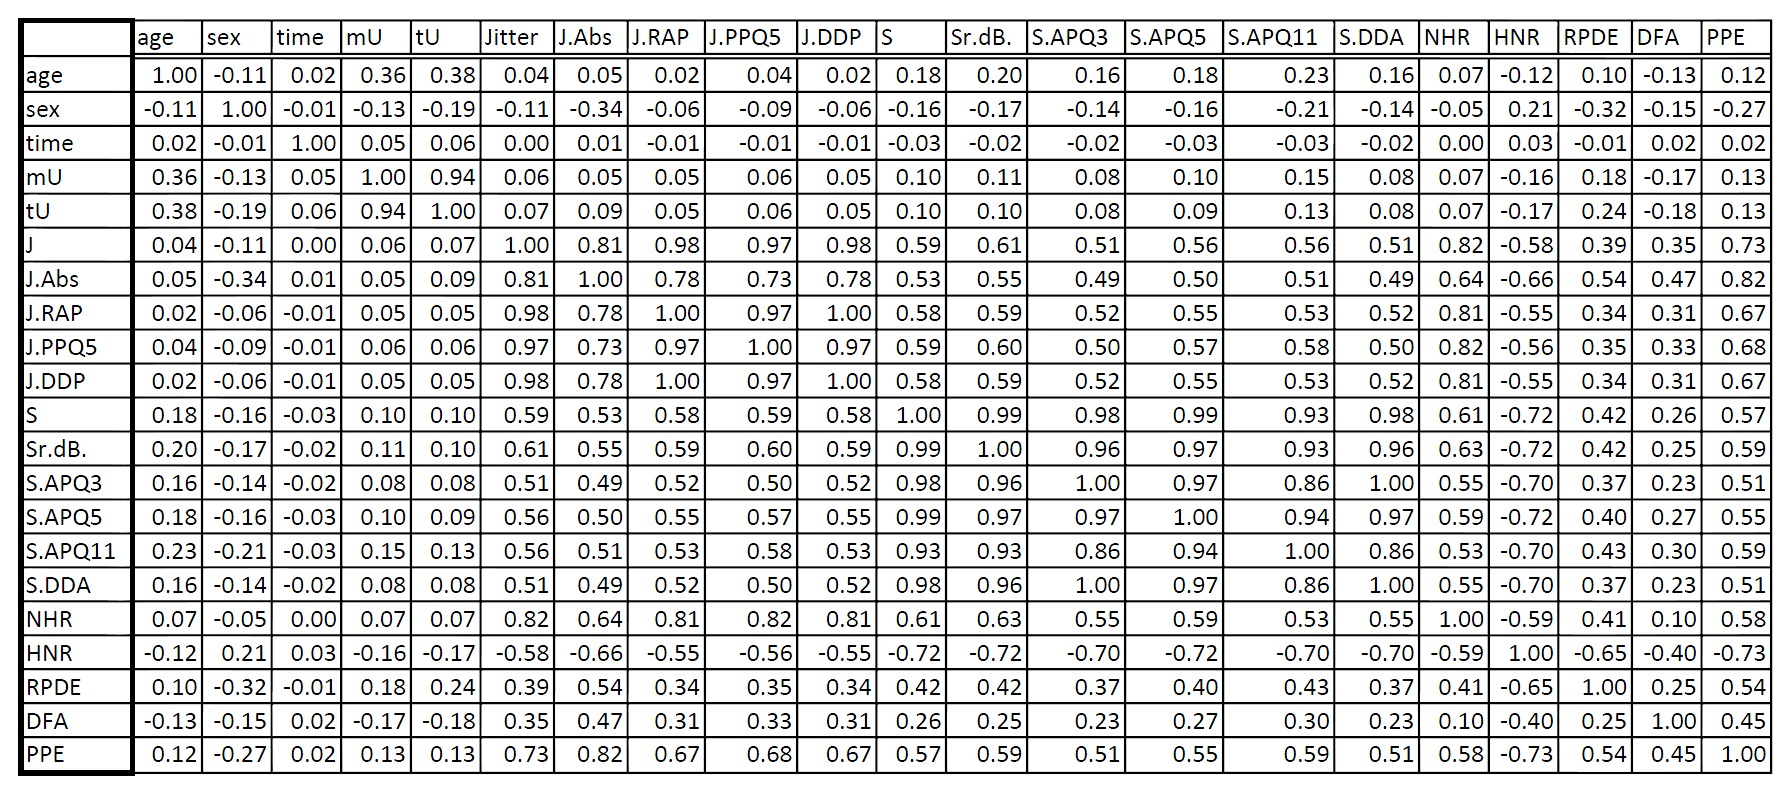
\includegraphics[width = 0.8\textwidth]{CorTable}

\caption{A table showing correlations of all predictors to each other. In this table, ``S'' stands for Shimmer and ``J'' stands for Jitter. ``mU'' and ``tU'' are motor and total UPDRS scores, respectively.
Note that the highest linear correlation to any one predictor is still very low ($<$0.15)}

\end{figure}


%%%%%%%%%

\begin{figure}[h]

\centering

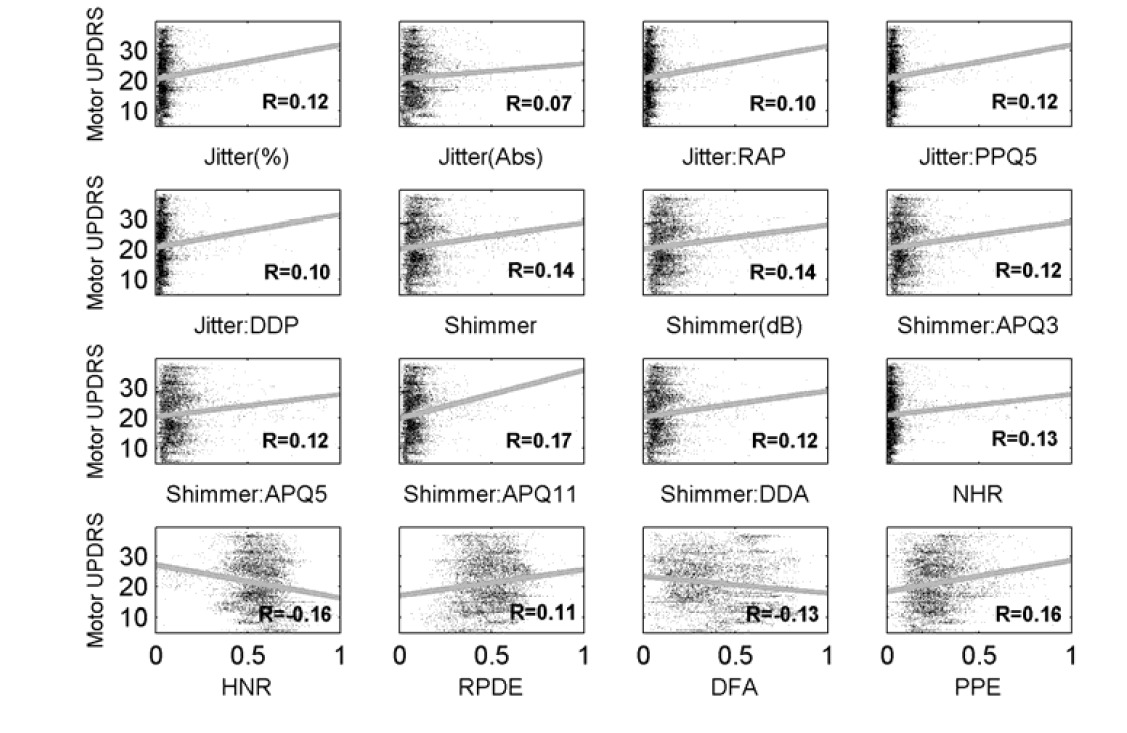
\includegraphics[width=0.8\textwidth]{regressionplotpredictors}

\caption{A plot of all predictors against motor UPDRS scales, take from Tsanas et. al.\cite{main} There is very little direct linear correlation in these plots, which precludes visually inspecting and choosing
appropriate variables.}

\end{figure}

%%%%%%%%%%%%


Other starting points for predictor selection include a stepwise forecast. In stepwise forecasting, predictors are added or removed one at a time, with the goal of creating the most accurate model possible
with the fewest number of variables. Unfortunately, since variables are added or removed one at a time, these algorithms can miss models that involve different combinations of
variables.

While we considered all these initial tools (and the issues that come with them), we ultimately rejected them for one simple reason: they are unnecessary. If we treat all Jitter measurements as one variable
and all Shimmer measurements as another, we wind up with only 7 voice-based predictors: Shimmer, Jitter, NHR, HNR, RPDE, DFA, and PPE. This is few enough to where manually
trying many different models (or brute-forcing) is a viable solution.

We started with the model obtained by Tsanas et. al., which had an mean absolute error (MAE) of 7.95 $\pm$ 0.19 under CART methods. Since the data set for this model has been slightly modified,
we first took their models and compared them against our results. We found that their models had a significantly higher error under least-squares regression than our models:
approximately 6.2 versus 6.8. We used our error of 6.2 with their formula as a starting point. By varying which predictors were included, we were able to decrease the error,
though not significantly. 

Once we started including age in our models, we were able to significantly decrease the mean error, although the extreme error cases remained the same. By adding consecutive 
powers of age up to the fourth power (i.e. $age^2$, $age^3$, $age^4$), we were able to reduce the MAE to below 5, both in and out of sample. However, we
discovered that with age as a predictor, Jitter and Shimmer no longer affected the MAE. Accordingly, we took them out of the model. We have not yet analyzed the effects of these
variables on the extreme error cases (which go up to $\pm17$), so it is possible that they will still be included in the model. Additional powers of age appear to increase the error,
and a Taylor Series expansion of exp(age) about the mean of the age, which is roughly proportional to $1 + x  + x^2 + x^3 $\dots$ (x = age)$, performs worse than leaving age out as a 
predictor. This suggests that only the first few powers of age have significant predictive power. Curiously, the $age^4$ term has a tiny coefficient from regression, but is responsible
for reducing the MAE from 5.5 to below 4. Why this is the case is currently unknown.

\section*{Model Performance}

Under 10-fold cross-validation, all our models were relatively stable. Our current model, which uses the first four powers of age, the first two powers of DFA, and HNR/NHR, has a
Mean Absolute error of 4.97, with a low variance. Curiously, in several thousand runs of cross-validations, the variance sometimes spikes to as high as 1. The reasons for this are
not yet clear, but it should be noted that, even within the current data set, the model sometimes seems to fail drastically (in perhaps 1 out of 500 cases). In 10000 runs of
10-fold cross validation, the out-of-sample Mean Absolute Error is 4.975, with a standard deviation (between cross validation runs) of 0.001.

We initially wondered if the completely linear nature of the interpolated data points was somehow affecting the model. To test this, we added noise to the samples: an error value taken from uniform and normal random variables.
Randomization of the data by adding values sampled from a U(-2,2) distribution did nothing to change the mean errors of the model, and the coefficients of each term did not change significantly, suggesting that the model was not dependent
on the perfectly linear nature of the samples.

Additionally, this model shows a roughly normally-distributed set of errors. Assuming that the errors are independent per patient, this result suggests that a least-squares regression is, in fact,
the appropriate method to use to fit this model (Figure 3).

\begin{figure}

\centering
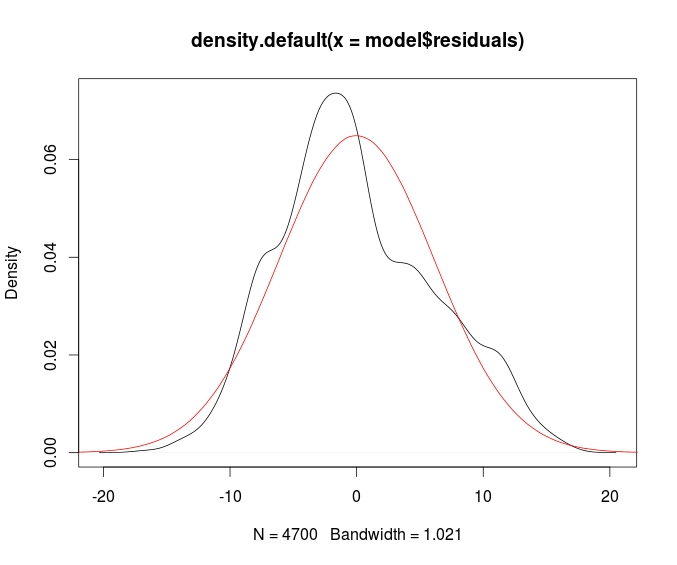
\includegraphics[width = 0.9\textwidth]{Error_Densities}

\caption{The residuals of the model (plotted in black) and a normal distribution with the same mean and variance (plotted in red). Note the asymmetry of the residuals, but rough agreement with the normal.
This suggests that the error is normally distributed, and that a least-squares regression is an appropriate modeling tool.}

\end{figure}

After we found our current model, we decided to attempt to improve on our model by doing a stepwise regression with our transformed variables. Forward stepwise regression shows that our model is more-or-less optimal for the variables we
are currently using. Curiously, a forward stepwise regression shows that the fifth and sixth powers of age are even more optimal, but there appears to be some sort of interaction between these higher powers of age and other predictors. 
Actually testing models with higher powers of age shows that they have significantly worse performance than models without any age dependence.

While this model does have extremely low errors, there are also some problems with it. First off, it does not segregate by gender, which may produce some unexpected results. Preliminary
data exploration has suggested that there is a significant difference between genders in respect to voice profiles, although we have not had the time to pursue these results further.

In addition, plots of the densities of the predictions show that the distribution for the predictions is more-or-less correct, but has a tendency to fall too close to the mode. This makes
some sense, since small voice distortions could be natural as aging progresses. %Look this up when you have time.
However, this also means that this model is not good for testing for Parkinson's disease early on (use for early screening).

The errors are also not completely random---even though they follow a normal distribution, they rise as a function of the motor UPDRS scores. While this definitely does not bode well for the model's performance,
we were unable to find a way to fix this problem. This suggests to us that the current model is somewhat incomplete.

\begin{figure}

\centering
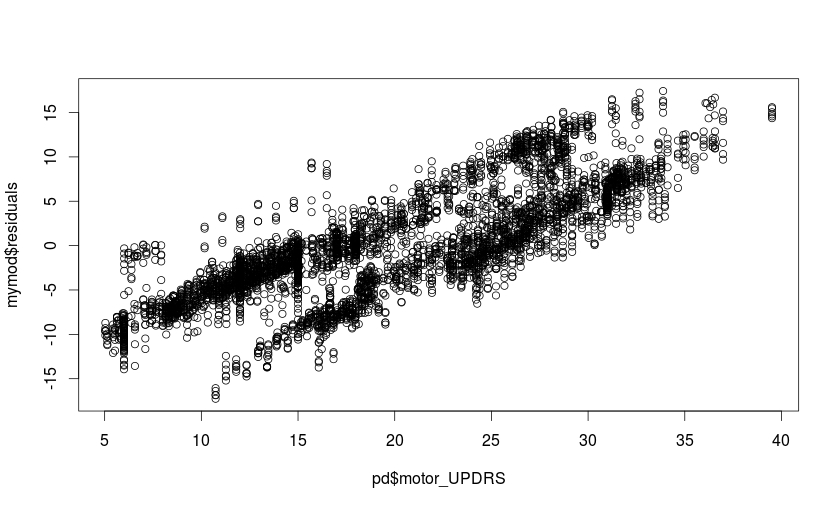
\includegraphics[width=0.9\textwidth]{resid_vs_motor}

\caption{The residuals of the model plotted against the motor UPDRS. Notice a strong correlation between the two. This suggests that the model that we are using is not quite complete. There is also a curious pattern of two
different lines, one vertically above the other. This implies that there are two groups of patients, and the errors tend to be different for each. We were unable to identify the nature of these groups in the time allotted.}

\end{figure}

Interestingly, a plot of the residuals against the motor UPDRS scores shows two distinct bands. This suggests that there is some way to categorize whether the residual will be higher or lower for a particular data point.
Unfortunately, we were unable to identify what causes this.

In an attempt to address all the above issues, we have preliminarily identified several possible relationships between these predictors and are working on breaking the data down into subgroups (for instance,
DFA seems to be much more predictive of PD in females than males). However, we have not made much headway as of this time.

\section*{Powers of Age}

One thing we found interesting while creating our models was the prevalence of powers of age. When we analyzed one of our initial models, based off of only of linear, nontransformed predictors, we found
that the ages were behaving quite strangely in the data points with larger error. To fix this, we initially added a second power of age, i.e. $age^2$. This reduced the error slightly. We then added a third power 
of age, and reduced the error even further. When we added a fourth power of age, the error dropped by a large amount (as much as adding the squared and cubed term together). A fifth power of age, however, reduced the performance of the model, and a sixth power made it even worse. This behavior was unexpected, and we spent
a large amount of time investigating it.

We attempted to determine whether this was frivolous behavior, perhaps resulting from overfitting or being dependent on the
interpolated nature of the data. Initially, we used a simple n-fold cross validation to rule out overfitting. We found that even under three-fold validation,
the model was remarkable stable. We also tried adding samples from the distributions U(-2,2) and Normal(mean=0, sd = 2). Neither of these measures caused any
decrease in model performance.

We then tried to use stepwise forecasting to predict the importance of the new transformed variables. Invariably, the fourth power of age always came out
as the most predictive variable, followed by the other powers of age and the other variables in our model. When we tried forward forecasting the higher powers of 
age (5, 6, 7), we found that they would always be ranked most predictive. However, the order of the other variables would become scrambled, and attempting to make
a model with the formula given by the stepwise regression always resulted in a higher error.

We have summarized our results in the table below. The formula used is motor\_UPDRS ~ (powers of age) + DFA + DFA$^2$ + DFA$^3$ + HNR + NHR, where powers of age are given in
the table (e.g. 1,3,4 = $age + age^3 + age^4$).

\begin{table}

\centering
\begin{tabular}{l | c}
Powers of Age & Mean Absolute Error\\
\hline \hline
1 & 5.89095\\
\hline
1,2 & 5.759798\\
\hline
1,3 & 5.734606\\
\hline
1,4 & 5.711099\\
\hline
1,3,4 & 5.456527\\
\hline
1,2,3 & 5.390792\\
\hline
1,2,3 &  5.386595\\
\hline
1,2,3,4 & 4.978422\\
\hline
1,2,3,4,5 & 4.985307\\
\hline
1,2,3,4,5,6 & 5.002124\\
\hline
\end{tabular}

\caption{A table of out-of-sample Mean Absolute Errors, obtained using a model of HNR, NHR, the first three powers of DFA, and the powers of age listed in the table. Notice how sharply the MAE drops after the addition of the 4th power, and that subsequent powers of age do nothing to improve it.}

\end{table}

All results in this table were taken from running 10-fold cross validations. Notice that only the first four powers of age seem to be significantly correlated with
the UPDRS, and that all four powers are necessary to reach the lowest MAE.

We conclude that somehow, the first four powers of age are strongly predictive of Parkinson's Disease in our model. Whether this will turn out to be the source
of the problems with this model (poor predictive power for low-UPDRS scoring patients) remains to be seen.


%%%%
%If we have more things to do with stepwise forecasts, they'll end up going here.
%%%%

\section*{Conclusion}

We have developed a model which can fairly accurately predict the severity of Parkinson's disease based 
upon several voice predictors.. This model does an excellent job of predicting motor UPDRS scores in patients with mild
Parkinson's. However, it lacks the early screening ability needed by an ideal test. 

The data also does not include several significant age groups: patients with a motor UPDRS of over 50 (advanced PD), people significantly under the
age of 45, and healthy patients. This means that, given a large abundance of any of these, the model could possibly fail (and indeed, may be likely to
fail in the case of advanced Parkinson's Disease).

The importance of the fourth power of age in this model is fairly interesting, and could arise from several factors. It could be a simple case of overfitting.
However, adding additional degrees of age (e.g. $age^5$, $age^6$) \textit{raises} the MAE, and so this seems unlikely. We have also explored the possibilty that
this is part of a Taylor Series expansion of another function about the median/mean of the age. All attempts resulted in a model that performed worse
than one without an age term. We are forced to conclude that a fourth power of age is somehow significantly correlated with the extent of Parkinson's Disease
in this model. Whether it is the correct model, or even whether it directly causes the flaws in this model (inability to predict low-level PD) remains to be seen.

Several factors also point to the possibilty of making gender-specific models. 

Ultimately, we have explored the effects of age on the severity of Parkinson's Disease, and come up with a model that includes several significant powers of age.
The correlation of these powers of age on UPDRS appear to be real and not caused by faulty modeling, as evidenced by the various stability tests we have run on the model.
This is not at all expected, and suggests that future exploration could be done in this area.



\bibliographystyle{plainnat}
\bibliography{biblio}




\end{document}

